\documentclass[runningheads,a4paper]{llncs}
\usepackage[T1]{fontenc}
\usepackage{graphicx,booktabs,amsmath}
\usepackage[hidelinks]{hyperref}
\title{ToolScope: Inspecting MCP Tool Discovery and Description-Edit Tradeoffs}
\titlerunning{ToolScope: Inspecting MCP Tool Discovery}
\author{Herender Kumar}
\authorrunning{H. Kumar}
\institute{Independent Researcher\\
\email{herender121112@gmail.com}}
\begin{document}
\maketitle
\begin{abstract}
ToolScope is an interactive workbench for inspecting Model Context Protocol (MCP) tool discovery. It connects retrieval comparisons, chronological agent traces and capability-level evidence, then measures how frozen description edits change ranks and coverage. A fixed LiveMCPBench snapshot supplies 525 tools and 95 tasks. The workbench compares six retrieval configurations and exposes 665 recorded trajectories. Replay reproduces all 1,611 original search shortlists. An exploratory repair study evaluates individual and joint edits, including translation controls, and reports gains alongside regressions. Diagnostic categories are rule-based hypotheses without independent expert validation. The demonstration helps MCP developers and retrieval researchers inspect missed capabilities and assess edits under a specified query, retriever and cutoff.
\keywords{Tool retrieval \and Model Context Protocol \and Interactive evaluation}
\end{abstract}

\section{Purpose and Positioning}
A useful tool may never enter an agent's shortlist, an available tool may be used unsuccessfully, or an external service may fail. Aggregate task-success scores cannot distinguish the supporting observations. Tool-definition quality scores also do not establish discoverability for a particular need. ToolScope connects retrieval comparisons, recorded searches and calls, and measured edit effects.

The intended users are MCP developers and tool-retrieval researchers. The contribution is the connection between saved evidence, capability-level drill-down and edit tradeoffs. The gateway is instrumentation: RAG-MCP studies retrieval before selection~\cite{ragmcp}, and Smart MCP Proxy (\texttt{mcpproxy-go}) provides discovery and routing~\cite{proxy}. Glama's TDQS~\cite{tdqs}, MCP Playground~\cite{playground} and ToolRank~\cite{toolrank} offer complementary quality or inspection tools. We claim no superiority over them.

LiveMCPBench supplies multi-server tasks and already analyzes failures by component~\cite{live}. ToolRet motivates evaluating whether all required tools are retrieved~\cite{toolret}. Hasan et al. study description augmentation and its effects on agent performance and cost~\cite{smelly}. Tool-DE shows that simple document expansion improves tool retrieval~\cite{toolde}; AgentCheck is a reproduce--intervene--mitigate workbench for MCP agents~\cite{agentcheck}. ToolScope centers on catalog retrieval: it shows how an edit's gains and regressions depend on retriever, query and cutoff, without assigning unique causal responsibility.

\section{System and Evidence Model}
\label{sec:system}
\textbf{Fixed data and retrieval.} The LiveMCPBench snapshot (commit \texttt{36a51a1}) contains 69 servers and 525 tools, versus 70/527 in its paper. IDs include server and tool name. The answer key, frozen at \texttt{gold-v1} before retrieval experiments, maps 95 tasks to 255 capabilities. Acceptable tools perform the same job with the same kind of input/output. Strict judgments use annotated targets; capability scoring accepts recorded equivalence classes.

The six configurations are BM25, BGE-base semantic retrieval, ToolRet-trained E5, reciprocal-rank fusion of BM25 and ToolRet (constant 60), MS MARCO MiniLM-L6-v2 reranking of the hybrid top 30, and server-first retrieval through five selected servers. ToolRet follows its evaluation configuration (mean pooling and recorded query prefix). Retrieval models are local and CPU-compatible; historical agent runs also include remote models.
\textbf{Two query scopes.} Original task-question rankings measure benchmark discovery. Agent-search evidence instead uses recorded queries and cutoffs in event order. Seven agent--strategy configurations each contribute 95 final trajectories: 665 total, with 1,611 searches at cutoff five and 1,132 distinct query strings. Replaying each distinct query through six retrievers yields 6,792 measurements, zero errors and exact reproduction of all original-strategy shortlists. This verifies consistency, not diagnostic validity.

Thirty-eight search responses were truncated; exposure requires an untruncated tool card. Calls are linked to earlier exposure, not to an offline ranking of the full question. Present-day retrievability does not establish historical exposure. The interface separates these scopes and preserves insufficient evidence: 50 of 1,785 agent-capability records remain unassigned.

\textbf{Hypotheses and provenance.} The taxonomy retains retrieval miss, ranking confusion, description-repairable miss, agent selection error, composition error and environment failure. Rules inspect retrieval, selection and execution evidence; external failures take precedence. Current agent-search analysis does not assign description or composition faults from task-question proxies. Description rescues belong to their measured query, strategy and cutoff. Cases expose the rule, acceptable tools, outcome source and evidence. These categories lack independent expert validation.

\textbf{Implementation.} A stateless FastMCP gateway exposes \texttt{search\_tools} and \texttt{call\_tool}, with asynchronous downstream calls and logged BM25 fallback on retrieval failure. Versioned JSONL logs and result artifacts feed FastAPI and React. Charts read saved measurements; exported case membership preserves each cohort through pagination. Docker Compose packages API, UI and an optional gateway. Indexes stay read-only; what-if runs in memory and writes nothing.

\section{Interactive Workflow}
\textbf{Compare.} Users inspect retrieval metrics and per-question rankings, separating strict relevance from capability completeness and context size. All configurations use the same catalog and answer key. Comparisons keep their query and cutoff.

\textbf{Failures.} Users select a run and hypothesis segment, then open a capability case. Search queries, returned IDs, raw arguments, saved result excerpts, errors and final answers support inspection of exposure before a call, argument validity and execution outcome. Truncation, unassigned coverage and human/judge provenance remain visible. Call success does not prove capability completion.

\textbf{Tool health and what-if.} Users inspect definitions, parameter documentation and misses, load a frozen query-blind rewrite or edit a description, then measure original/edited ranks under BM25 and semantic retrieval (Fig.~\ref{fig:whatif}). An interactive edit informed by the displayed task is exploratory, not a new query-blind experiment. The accompanying repair report measures joint edit sets and collateral losses rather than adding independent single-edit gains.

\begin{figure}[t]
\centering
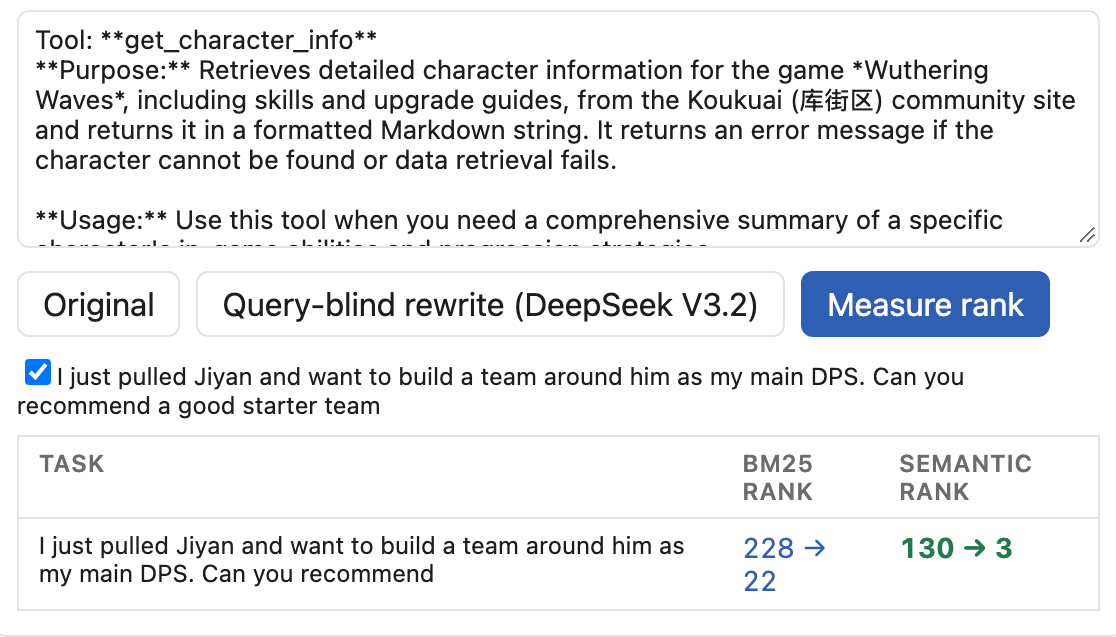
\includegraphics[width=0.72\textwidth]{figures/ui_whatif.png}
\caption{What-if editor for \texttt{wuwa-mcp/get\_character\_info}, whose original description is Chinese-only. The frozen rewrite was generated from tool metadata only, never a task query; measured in memory for the shown task, it moves the tool from rank 228 to 22 (BM25) and from 130 to 3 (semantic).}
\label{fig:whatif}
\end{figure}

\section{Measured Evidence}
\textbf{Retrieval comparison.} Table~\ref{tab:retrieval} reports results on 95 task questions. Recall, nDCG and MRR use strict judgments. Completeness requires an acceptable tool for every capability, adapting ToolRet's criterion~\cite{toolret}. Semantic nDCG@10 improves by 0.076 over BM25, but its Bonferroni-corrected $p=0.066$ exceeds 0.05. No configuration differs significantly from BM25 after correction for five paired comparisons. This does not establish equivalence.

\begin{table}[t]
\setlength{\tabcolsep}{3pt}\small
\begin{minipage}[t]{0.5\textwidth}\centering
\caption{Saved retrieval results on 95 task questions. C: capability completeness. No corrected significance threshold is met.}
\label{tab:retrieval}
\resizebox{\linewidth}{!}{\begin{tabular}{lrrrr}\toprule
Configuration & R@10 & nDCG@10 & MRR@10 & C@10\\\midrule
bm25 & 0.418 & 0.347 & 0.444 & 0.232 \\
semantic & 0.504 & 0.423 & 0.523 & 0.274 \\
toolret & 0.462 & 0.376 & 0.469 & 0.242 \\
hybrid & 0.458 & 0.376 & 0.475 & 0.253 \\
rerank & 0.430 & 0.347 & 0.427 & 0.232 \\
server\_first & 0.439 & 0.359 & 0.423 & 0.295 \\
\bottomrule\end{tabular}
}
\end{minipage}\hfill
\begin{minipage}[t]{0.47\textwidth}\centering
\caption{Joint edit sets at cutoff ten. Cap: capabilities found (of 255); Tasks: complete-task discoveries (of 95), not agent task success.}
\label{tab:repair}
\resizebox{\linewidth}{!}{\begin{tabular}{lrrrr}\toprule
& \multicolumn{2}{c}{BM25} & \multicolumn{2}{c}{Semantic}\\
Edit set & Cap & Tasks & Cap & Tasks\\\midrule
Original & 98 & 22 & 119 & 26 \\
Translation (12) & 103 & 22 & 127 & 27 \\
Structured (same 12) & 102 & 25 & 126 & 27 \\
Structured (43) & 116 & 27 & 129 & 27 \\
\bottomrule\end{tabular}
}
\end{minipage}
\end{table}

\textbf{Description interventions.} We evaluate 43 structured rewrites selected from known misses, with translation controls for 12 Chinese-containing originals. Each single edit is measured across all 95 questions, alongside joint translation, matched-12 structured and all-43 structured conditions. The study covers 91 scenarios and 17,290 query-level measurements across two retrievers at cutoffs five and ten. Saved-baseline, unchanged-description and historical-probe checks find zero mismatches.


Table~\ref{tab:repair} reports joint effects. All 43 structured edits change complete-task discovery from 22 to 27 for BM25 and 26 to 27 for semantic retrieval. The semantic net gain includes two newly complete tasks and one lost task; it gains 13 capabilities and loses three. Translation alone reaches 27 complete-task discoveries for semantic retrieval and leaves BM25 at 22.

\section{Demonstration and Limits}
The demonstration follows three cases: an exposed-but-not-called tool with its search/call evidence; a measured description intervention; and a joint-edit regression alongside gains. In the second case, the WuWa character-info tool moves semantic rank from 130 to 10 under translation and to 3 under a structured edit. BM25 ranks are 228, 228 and 22. Translation meets the semantic top-ten cutoff but misses the top five. Visitors can also edit other descriptions in memory.

The repair study is exploratory: candidates came from known misses. Translations use Qwen outputs with corrections by an AI assistant; structured texts reuse DeepSeek outputs, so differences cannot isolate a model or prompt effect. An AI assistant's review flags faithfulness concerns in 22 of 43 rewrites, without human or execution checks. Discovery gains do not imply task-success gains.

Task-success judging does not validate diagnosis. The Kimi BM25 judge failed the predeclared agreement threshold, so its outcomes use author labels. Other judge outcomes retain their limited validation scope; Kimi semantic remains unvalidated. Saved traces stay inspectable if upstream services change. Demo video: \textbf{[VIDEO URL]}. Code: \textbf{[CODE URL]}.

\textbf{Use of AI tools.} Claude (Anthropic) helped implement the software and edit this paper. In the study, DeepSeek V3.2 judged task success and wrote the query-blind rewrites; a local Qwen2.5-7B produced translations. The author verified all numbers and references and takes full responsibility for the content.

\clearpage
\begin{thebibliography}{10}
\bibitem{ragmcp} Gan, T., Sun, Q.: RAG-MCP: Mitigating Prompt Bloat in LLM Tool Selection via Retrieval-Augmented Generation. arXiv:2505.03275 (2025). \url{https://arxiv.org/abs/2505.03275}
\bibitem{smelly} Hasan, M.M., Li, H., Rajbahadur, G.K., Adams, B., Hassan, A.E.: Model Context Protocol (MCP) Tool Descriptions Are Smelly! Towards Improving AI Agent Efficiency with Augmented MCP Tool Descriptions. arXiv:2602.14878 (2026). \url{https://arxiv.org/abs/2602.14878}
\bibitem{toolde} Lu, X., Huang, H., Meng, R., Jin, Y., Zeng, W., Shen, X.: Tools are under-documented: Simple Document Expansion Boosts Tool Retrieval. arXiv:2510.22670 (2025). \url{https://arxiv.org/abs/2510.22670}
\bibitem{agentcheck} Mazumder, A., Lia, N.J.: AgentCheck: A Reproduce--Intervene--Mitigate Workbench for LLM Agents over MCP. In: Proceedings of the 2026 Conference on Empirical Methods in Natural Language Processing: System Demonstrations, pp. 674--684. ACL, Budapest, Hungary (2026). \url{https://aclanthology.org/2026.emnlp-demos.64/}
\bibitem{live} Mo, G., Zhong, W., Chen, J., Yuan, Q., Chen, X., Lu, Y., Lin, H., He, B., Han, X., Sun, L.: LiveMCPBench: Can Agents Navigate an Ocean of MCP Tools? arXiv:2508.01780 (2025). \url{https://arxiv.org/abs/2508.01780}
\bibitem{toolret} Shi, Z., Wang, Y., Yan, L., Ren, P., Wang, S., Yin, D., Ren, Z.: Retrieval Models Aren't Tool-Savvy: Benchmarking Tool Retrieval for Large Language Models. arXiv:2503.01763 (2025). \url{https://arxiv.org/abs/2503.01763}
\bibitem{proxy} Smart MCP Proxy: mcpproxy-go. \url{https://github.com/smart-mcp-proxy/mcpproxy-go}. Accessed 3 Nov 2026
\bibitem{tdqs} TDQS: Tool Definition Quality Score, Specification 1.2. \url{https://tdqs.dev/spec}. Accessed 3 Nov 2026
\bibitem{playground} MCP Playground: Documentation. \url{https://www.mcpplayground.tech/docs}. Accessed 3 Nov 2026
\bibitem{toolrank} ToolRank: Agent Tool Optimization. \url{https://toolrank.dev/}. Accessed 3 Nov 2026
\end{thebibliography}
\end{document}
